\documentclass[11pt,letterpaper]{article}
\usepackage[margin=0.7in]{geometry}
\usepackage{graphicx,amsmath,amssymb,bm,mathrsfs,caption}
\usepackage[colorlinks=true,linkcolor=blue]{hyperref}
\captionsetup{font=small,labelfont=bf}
\setlength{\parindent}{0pt}
\emergencystretch=1.5em
\newcommand{\scrD}{\mathscr{D}}
\newcommand{\scrA}{\mathscr{A}}
\newcommand{\calH}{\mathcal{H}}
\newcommand{\calA}{\mathcal{A}}
\newcommand{\calB}{\mathcal{B}}
\newcommand{\calK}{\mathcal{K}}
\newcommand{\calM}{\mathcal{M}}
\newcommand{\lP}{\ell_P}
\newcommand{\Tr}{\mathrm{Tr}}
\newcommand{\ethop}{\eth}
\newcommand{\bareth}{\bar{\eth}}


\begin{document}
\textbf{Figure review: finite-state null-cone model}\par
\small Main figures 1--6; additional benchmarks 7--11. Captions match the manuscript.\normalsize
\begin{figure}[!ht]
\centering
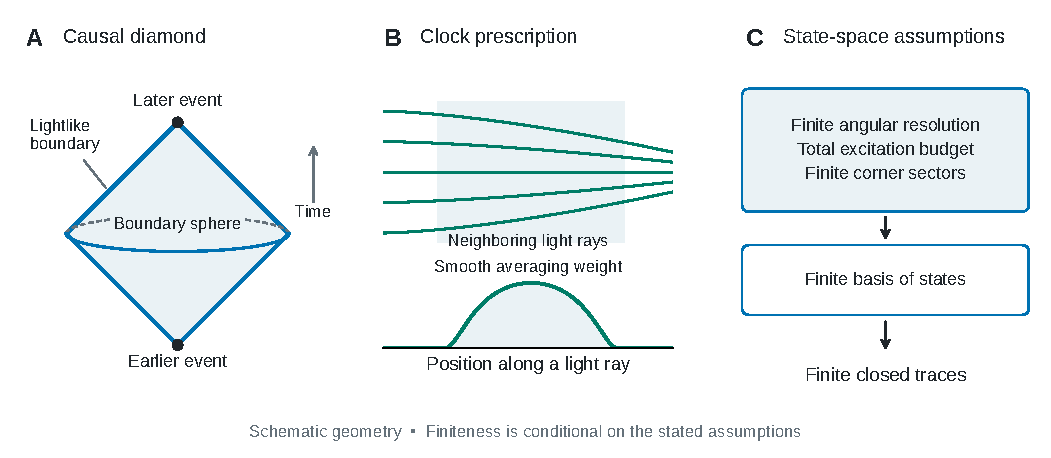
\includegraphics[width=\linewidth,height=6.6in,keepaspectratio]{figs/review_01_causal_diamond.pdf}
\caption{\textbf{From a region bounded by light to a finite model.} (A) The causal diamond contains events that can receive a signal from the earlier tip and send one to the later tip. The ellipse represents a spherical cross-section. (B) Neighboring light rays focus; the modified clock subtracts the vacuum contribution and averages over a smooth weight. Ray paths are schematic and the weight is the rescaled taper of Sec.~III\,B. (C) Finite angular resolution, a total excitation budget, and finite corner sectors supply a finite basis. Closed traces are finite as a consequence of these explicit assumptions.}
\label{fig:geometry}
\end{figure}
\clearpage

\begin{figure}[!ht]
\centering
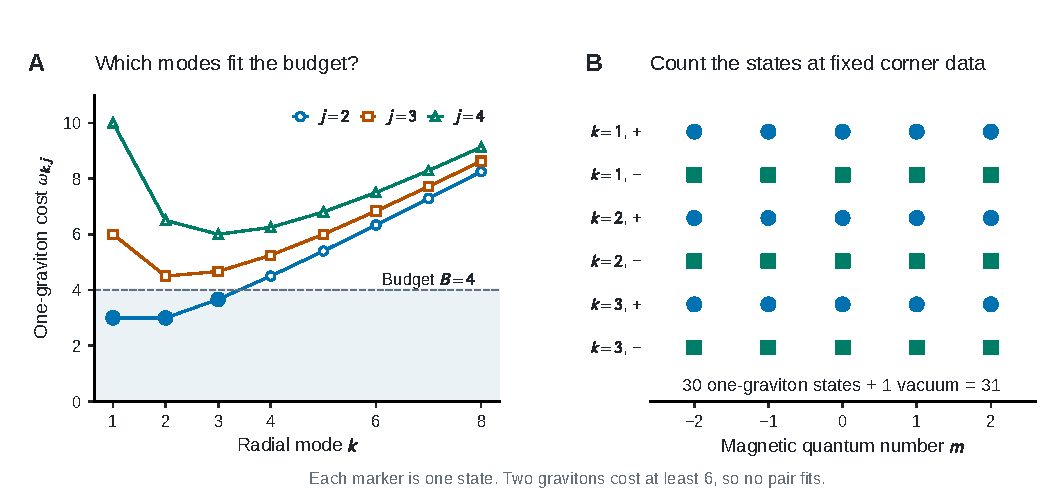
\includegraphics[width=\linewidth,height=6.6in,keepaspectratio]{figs/review_02_state_count.pdf}
\caption{\textbf{An exactly enumerable 31-state radiative sector.} (A) Discrete costs $\omega_{k,j}=k+(j-1)(j+2)/(2k)$ for three angular modes. Filled markers lie within the total budget $B=4$; only $(j,k)=(2,1),(2,2),(2,3)$ qualify, with costs $3,3,11/3$. Lines connect discrete values as guides. (B) Each marker is one one-graviton basis state: three radial modes, five magnetic substates, and two polarization labels ($+$ and $-$). The vacuum adds one state. Every two-graviton state costs at least six. The count fixes the corner sector and assumes $J_{\max}\ge2$.}
\label{fig:state_count}
\end{figure}
\clearpage

\begin{figure}[!ht]
\centering
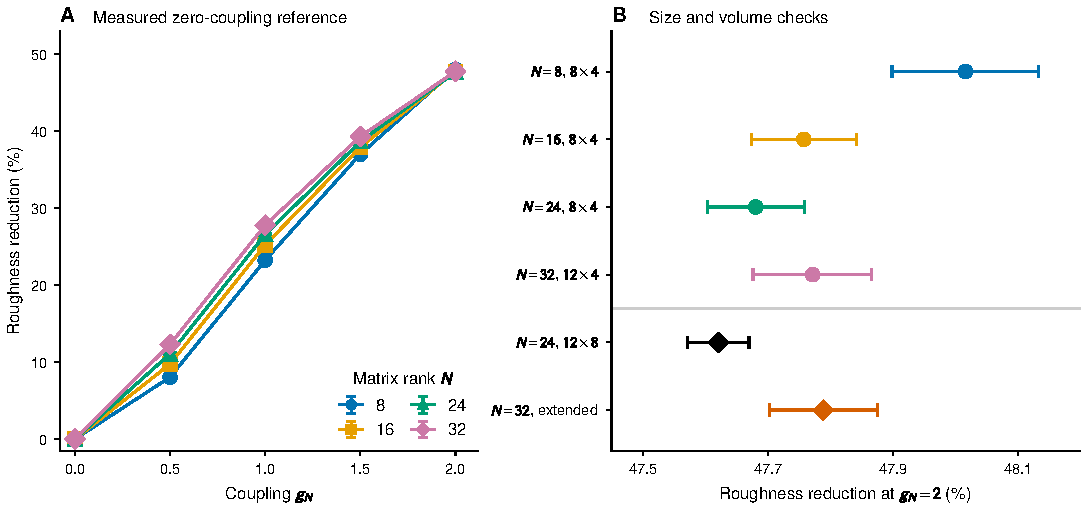
\includegraphics[width=\linewidth,height=6.6in,keepaspectratio]{figs/fig_followup_roughness.pdf}
\caption{\textbf{Coupling suppresses traceless matrix-field fluctuations.} (A) Mean dimensionless traceless matrix-field fluctuation $Q_2$ versus coupling. Colors and shapes identify matrix rank; lines guide the eye. Bars are $1.96$ times the archived Monte Carlo standard error, often smaller than the symbols. (B) Reduction $100[1-\overline Q_2(2)/\overline Q_2(0)]$, using a measured zero-coupling control at the same rank and lattice. The percentage axis is expanded to show size dependence. Bars are the archived approximate 95\% propagated ratio intervals. The four main coupled ensembles use 4--8 chains; the extended $N=32$ check uses 16 chains with 2000 draws per chain, and the $12\times8$ check uses eight with 700. All comparisons retain $\mu^2=0.25$ and $\lambda_4=0.1$. Intervals quantify sampling uncertainty, not model or discretization uncertainty.}
\label{fig:roughness}
\end{figure}
\clearpage

\begin{figure}[!ht]
\centering
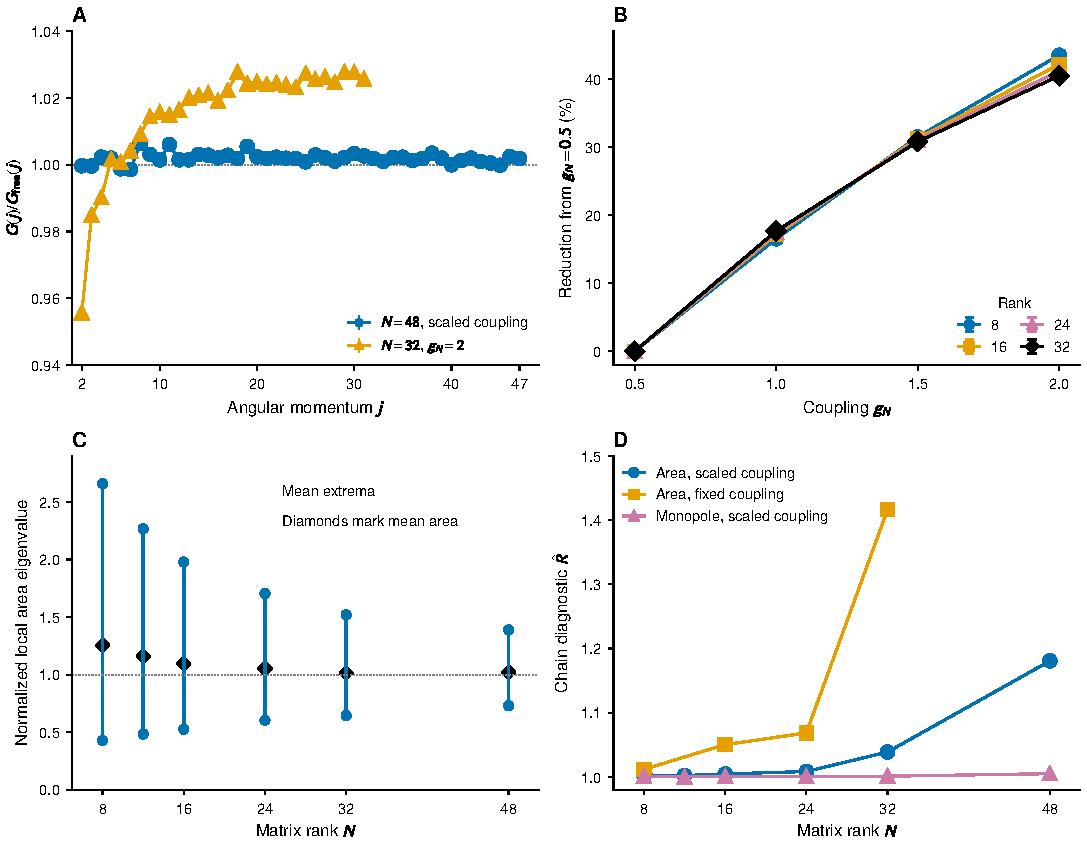
\includegraphics[width=\linewidth,height=6.6in,keepaspectratio]{figs/fig6_modal_b200_hmc.pdf}
\caption{\textbf{Sampling convergence depends on the observable.} Rank-normalized split-$\hat R$ for (A) roughness and (B) local mean area, with different horizontal scales. Values near one indicate agreement across split chains; the target is $\hat R<1.01$. (C) Bulk and tail effective sample sizes (ESS) for local mean area, on a logarithmic axis; the target is at least 400 for each. ``Global'' and ``+local'' identify the successive sampling schemes, with local collective moves added in the latter. The extended $N=32$ and $N=48$ runs use 16 chains with 2000 retained draws per chain; their couplings differ as specified in the text. The $N=24$, $12\times8$ test has eight chains with 700 draws. Its roughness passes the displayed targets while its area remains poorly mixed. These diagnostics do not prove stationarity.}
\label{fig:hmc}
\end{figure}
\clearpage

\begin{figure}[!ht]
\centering
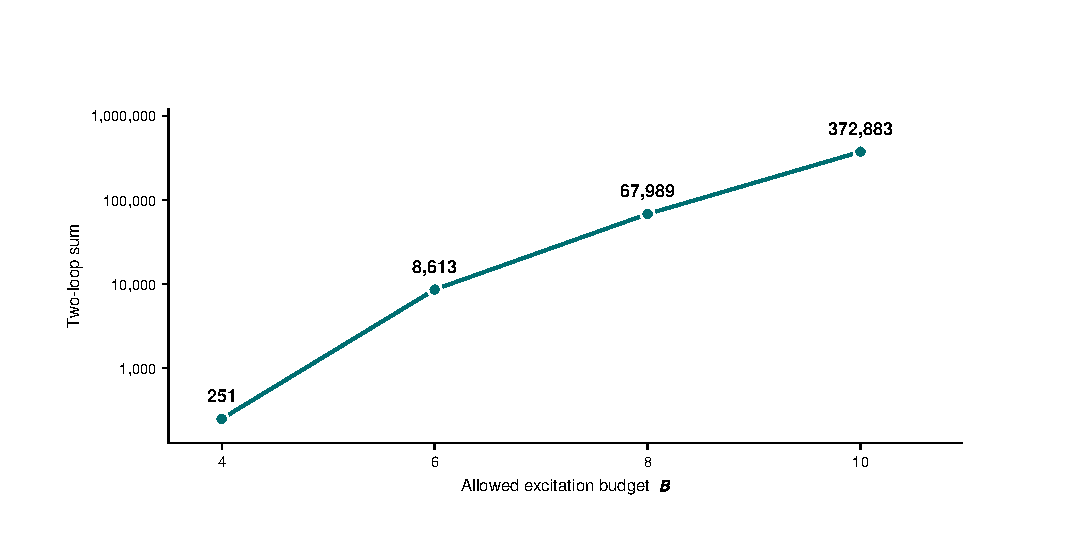
\includegraphics[width=\linewidth,height=6.6in,keepaspectratio]{figs/review_03_two_loop_budget.pdf}
\caption{\textbf{Finite resolution and cutoff removal are different questions.} (A) Archived one- and two-loop diagnostic integrals with fixed angular cutoff as the radial/time cutoff grows. The one-loop expression approaches its reference limit while the two-loop diagnostic grows. (B) The regulated two-loop sum at four single-mode cost cutoffs $\omega_{k,j}\le B$; labels give the admitted mode count. Both vertical axes are logarithmic and lines guide the eye. The many-particle projector also constrains total intermediate-state cost. These fixed-cutoff calculations do not establish a finite ultraviolet limit.}
\label{fig:budget_growth}
\end{figure}
\clearpage

\begin{figure}[!ht]
\centering
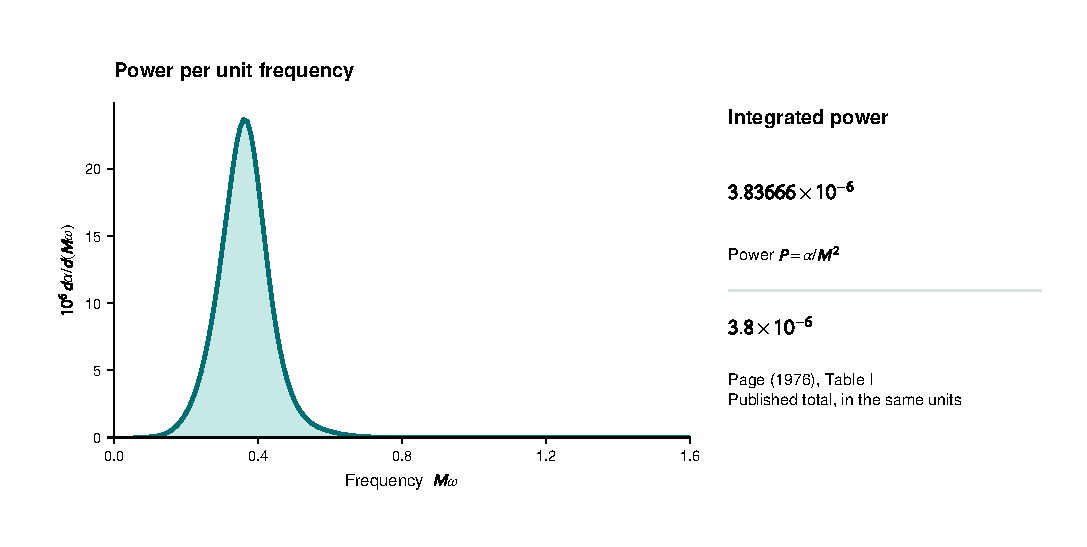
\includegraphics[width=\linewidth,height=6.6in,keepaspectratio]{figs/review_04_graviton_spectrum.pdf}
\caption{\textbf{A known Schwarzschild graviton-emission benchmark.} (A) Regge--Wheeler transmission probabilities for angular momenta $j=2,\ldots,6$. (B) The spectrum after thermal weighting and summation over both helicities. Its shaded integral gives $\alpha=3.83666\times10^{-6}$ and power $P=\alpha/M^2$ in units $G=c=\hbar=1$. The calculation uses 155 frequencies over $0.06\le M\omega\le1.60$ and 2400 radial tortoise-coordinate samples. Page's published total is $3.8\times10^{-6}$~(Page, 1976, Table I); extra precision of the numerical integral is not extra precision of that reference. The quadrupole supplies $99.06\%$ of the computed power. Agreement tests this scattering calculation, not a derivation of the full quantum theory.}
\label{fig:hawking}
\end{figure}
\clearpage

\begin{figure}[!ht]
\centering
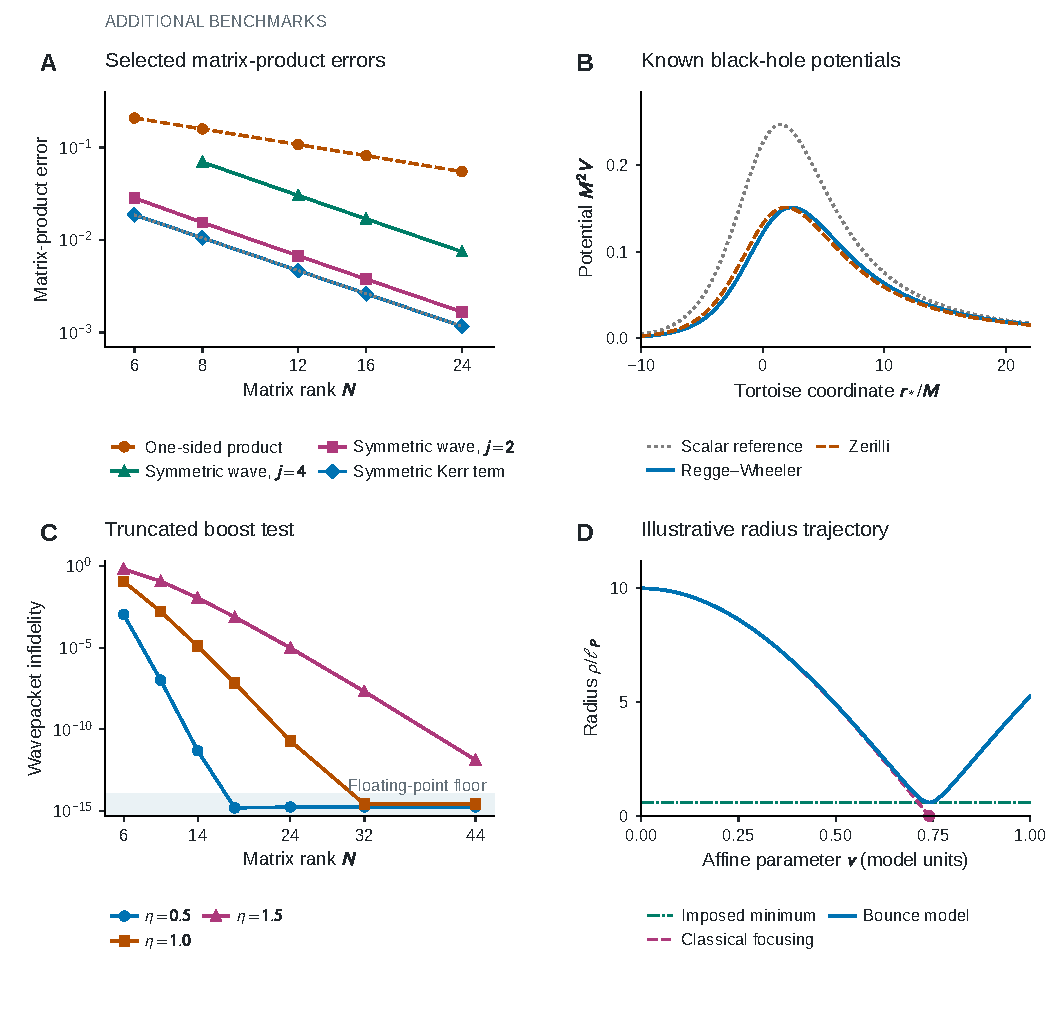
\includegraphics[width=\linewidth,height=6.6in,keepaspectratio]{figs/fig2_unified_matrix_gravity.pdf}
\caption{\textbf{Selected matrix and classical benchmarks.} (A) Errors in chosen Kerr and gravitational-wave matrix products versus continuum coefficients; the symmetric products decrease approximately as $N^{-2}$ over the tested range. (B) Known scalar, Regge--Wheeler, and Zerilli potentials at $j=2$. (C) Infidelity of truncated spin-2 boost wavepackets relative to the reference representation at three rapidities. The shaded range marks values near floating-point precision, not resolved evidence of exact covariance. (D) A classical focusing trajectory compared with an illustrative Ermakov--Pinney trajectory with imposed $\rho_{\min}=\sqrt{\ln3/\pi}\,\lP$. The classical curve stops at its caustic. This example does not derive singularity avoidance from the interacting matrix dynamics.}
\label{fig:unified}
\end{figure}
\clearpage

\begin{figure}[!ht]
\centering
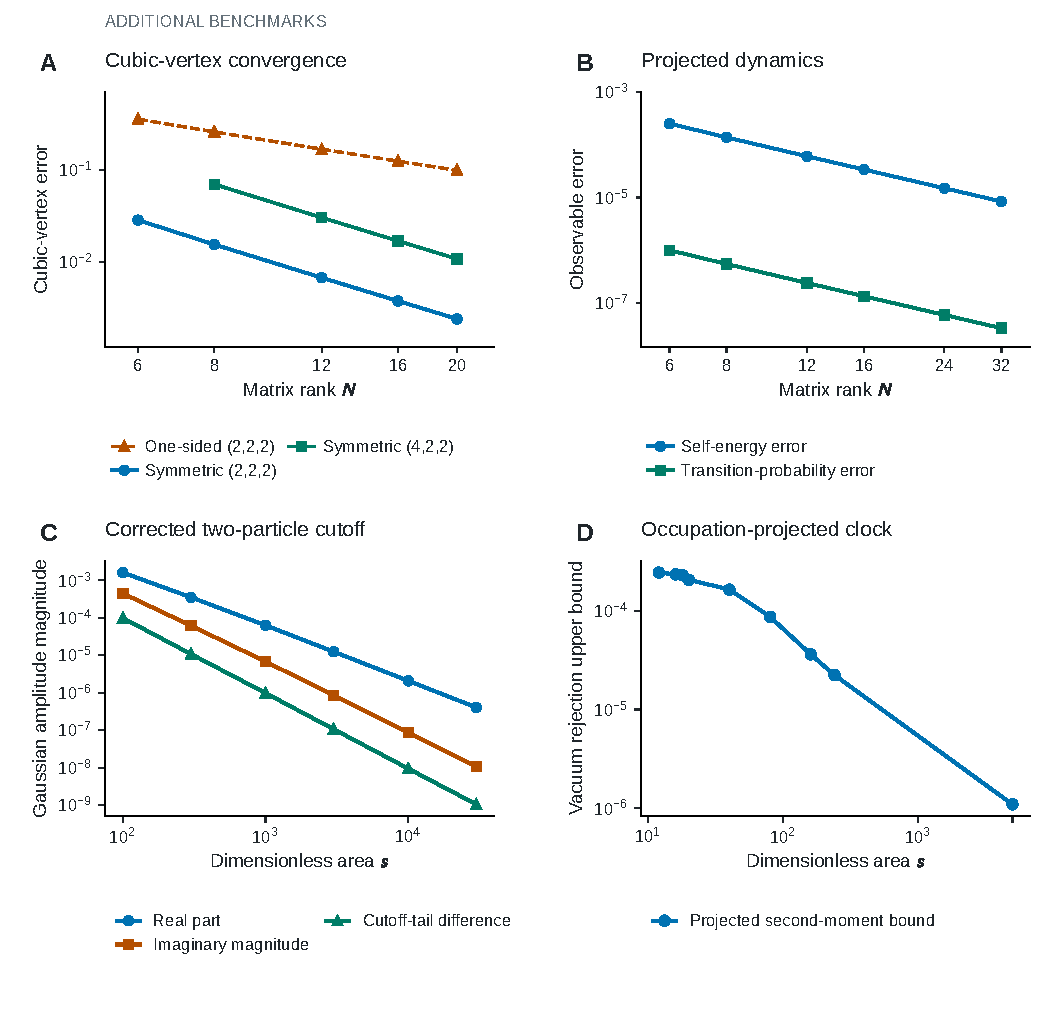
\includegraphics[width=\linewidth,height=6.6in,keepaspectratio]{figs/fig5_v2_unification_and_clock.pdf}
\caption{\textbf{Finite-model vertex, dynamics, amplitude, and clock tests.} (A) Cubic-vertex errors for one-sided and parity-symmetric matrix contractions. (B) Self-energy and transition-probability errors in the finite projected Hamiltonian example relative to its continuum-vertex counterpart. (C) The Gaussian pair sum with the corrected two-particle condition $2\omega_{k,j}\le B(s)=s$; the third curve is its difference from the radial-unrestricted reference. At $B=4$, no pair is allowed. (D) The recomputed second-moment upper bound on vacuum clock-projector rejection for the actual total occupation projector, with $B(s)=0.5s$, $J(s)=\lfloor\sqrt{s/\ln3}\rfloor$, and $\ell/u_{\mathrm{cl}}=2$. The $B=4$ vacuum has exactly zero rejection and is omitted from the logarithmic axis. The old fourth-moment and Chernoff curves do not apply to this compressed exponential and have been removed. Curves are numerical evaluations of bounds, not Monte Carlo observations. These tests have the model scope described in Sec.~III.}
\label{fig:v2}
\end{figure}
\clearpage

\begin{figure}[!ht]
\centering
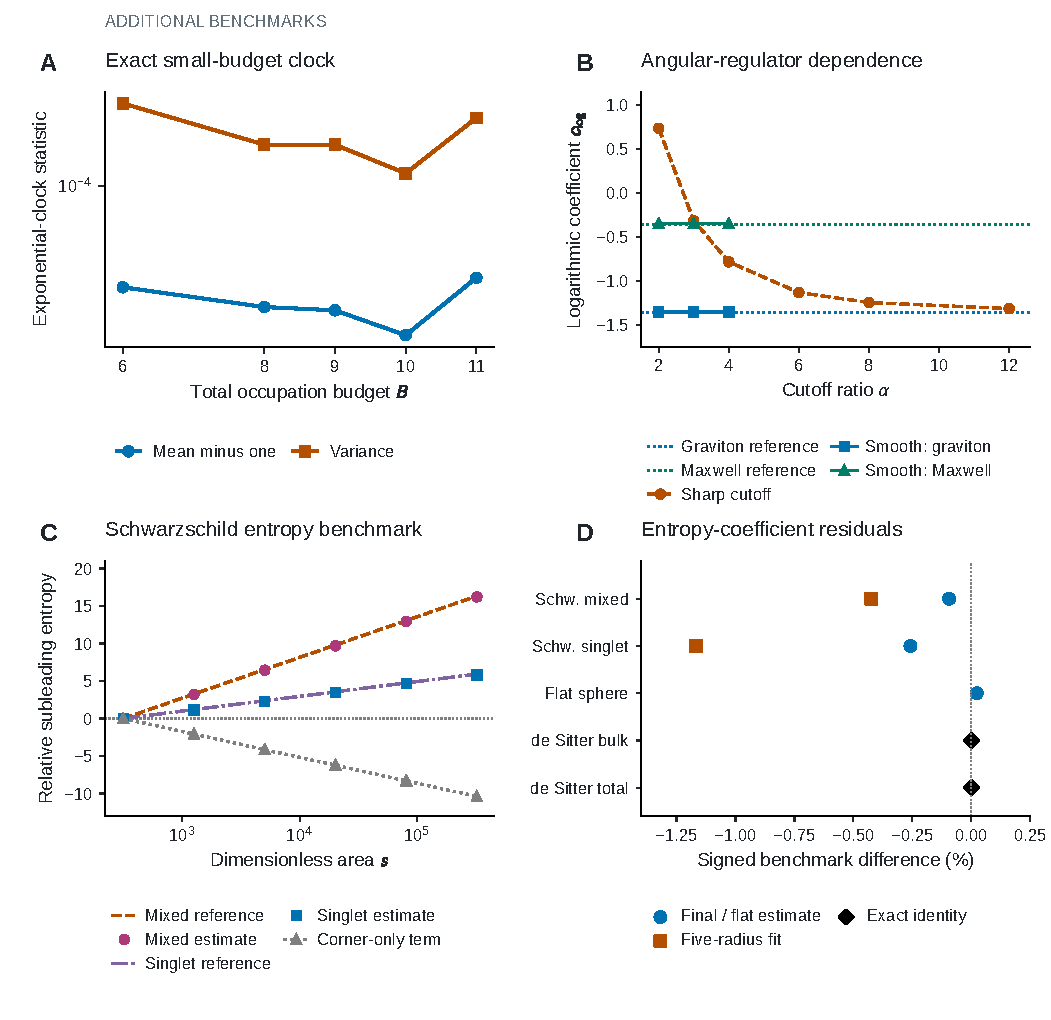
\includegraphics[width=\linewidth,height=6.6in,keepaspectratio]{figs/fig1_breakthrough_1loop.pdf}
\caption{\textbf{Clock and one-loop coefficient benchmarks.} (A) Exact vacuum means and variances of $e^{\Xi_{s,B}}$ for the occupation-projected clock at $s=2B$ and $B<12$. The plotted mean is shown as its excess above one. At $B=4$ both statistics are exactly zero and are omitted from the logarithmic axis. New states entering the budget prevent a monotone interpretation. (B) Extracted flat-space logarithmic coefficients under sharp and smooth angular regulators, compared with known graviton and Maxwell references. (C) Schwarzschild subleading entropy, with a common additive constant removed, compared with the $106/45$ mixed and $77/90$ singlet coefficients. (D) Signed residuals $100(c_{\mathrm{est}}-c_{\mathrm{ref}})/|c_{\mathrm{ref}}|$: final-doubling estimates, five-radius fits, and exact coefficient identities are distinguished by marker. Known heat-kernel inputs and identities make these consistency checks; the plot is not an independent nonperturbative entropy derivation.}
\label{fig:1loop}
\end{figure}
\clearpage

\begin{figure}[!ht]
\centering
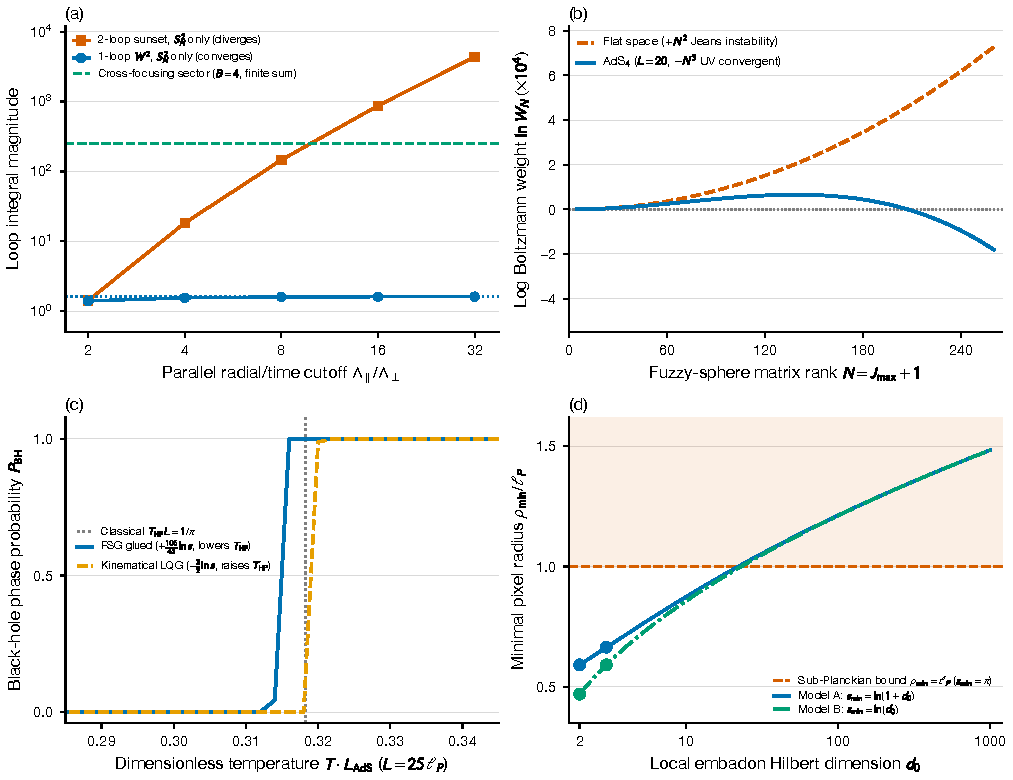
\includegraphics[width=\linewidth,height=6.6in,keepaspectratio]{figs/fig3_uv_completion.pdf}
\caption{\textbf{Regulator and thermodynamic model examples.} (A) Transverse-only loop diagnostics; the horizontal line is the separately regulated single-mode sum at $B=4$. (B) Rank weights computed from the assumed entropy and energy functions for flat space and AdS, with $\beta=L=20$ in Planck units. (C) Black-hole probabilities in the rank-sum model at $L=25\,\lP$, comparing two input logarithmic entropy coefficients; the vertical line is the classical temperature $TL=1/\pi$. (D) Pixel radius as a function of the postulated local corner dimension under two entropy prescriptions. The shaded region violates the imposed radius criterion $\rho_{\min}\le\lP$. These are conditional model calculations, not a derivation of ultraviolet completion or a unique corner spectrum.}
\label{fig:uv}
\end{figure}
\clearpage

\begin{figure}[!ht]
\centering
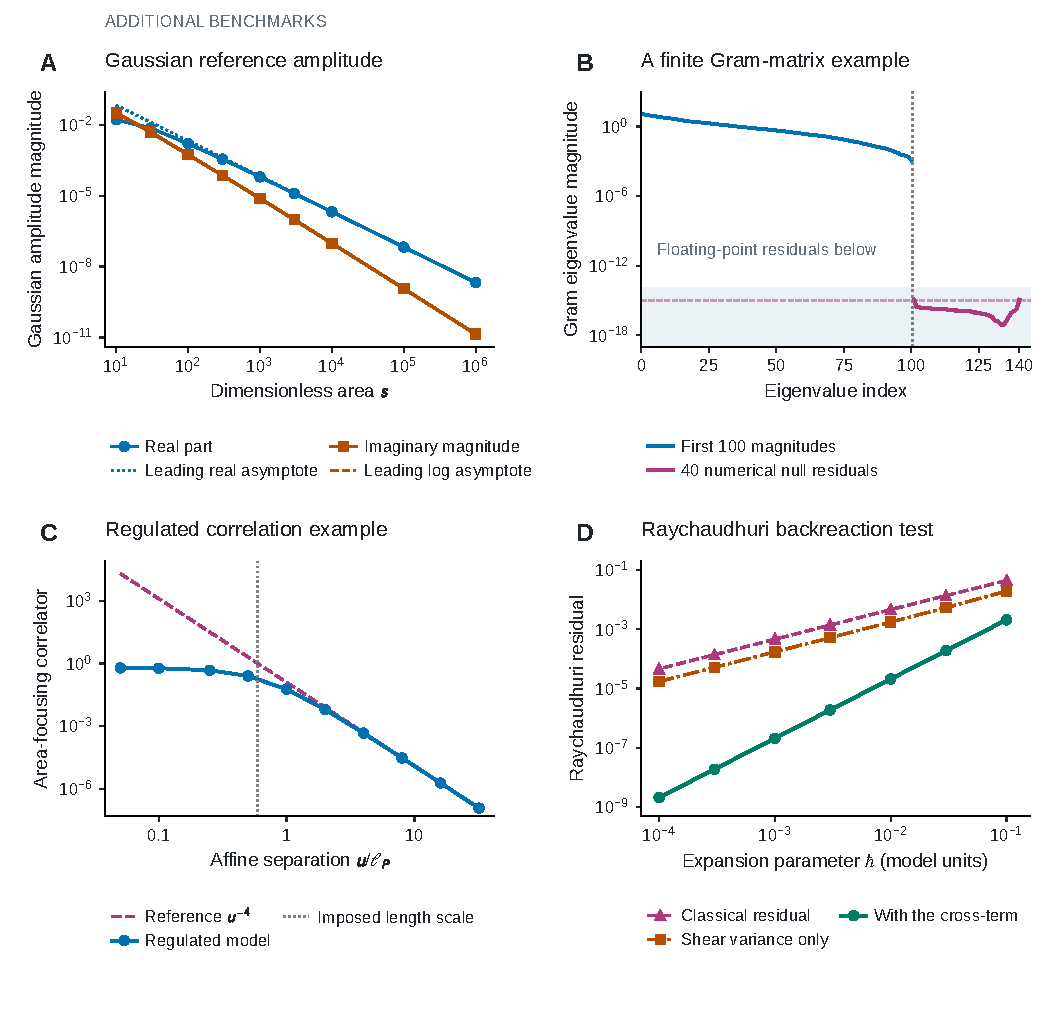
\includegraphics[width=\linewidth,height=6.6in,keepaspectratio]{figs/fig4_original_resolution.pdf}
\caption{\textbf{Gaussian and finite-matrix consistency examples.} (A) A radial-unrestricted Gaussian pair reference with finite angular cutoff, compared with its leading real and imaginary asymptotes. The budget-projected sum is shown separately in Fig.~\ref{fig:v2}(C). (B) Eigenvalue magnitudes of the Gram matrix for 140 constructed fillings in a 100-dimensional operator space. Forty residual magnitudes lie near floating-point precision; the rank bound follows from the chosen algebra. (C) A regulated area-focusing correlator and its large-separation $u^{-4}$ reference. (D) A one-generator Raychaudhuri calculation: retaining the metric--shear cross-term changes the residual scaling from approximately first to second order in the expansion parameter. These examples do not establish a dynamical resolution of topology sums, emergent spacetime, or complete four-dimensional backreaction.}
\label{fig:orig}
\end{figure}
\clearpage
\end{document}
